\documentclass[UTF8,openany,zihao=5]{ctexbook}

% 论文版面要求:
% 统一按 word 格式A4纸(页面设置按word默认值)编排、打印、制作。
% 正文内容字体为宋体;字号为小4号;字符间距为标准;行距为25磅(约0.88175cm)。

%%%%% ===== 页面设置
\usepackage[a4paper,top=3cm,bottom=3cm,left=2.5cm,right=2.5cm,%
            ]{geometry}
\usepackage{booktabs}
\usepackage{bicaption}
\captionsetup[figure][bi-first]{name=图}
\captionsetup[figure][bi-second]{name=Fig.}
            
\captionsetup[table][bi-first]{name=表}
\captionsetup[table][bi-second]{name=Tab.}


\usepackage{enumitem}
\setlength{\parindent}{2em}
%默认的弹性间距会导致文中某些排版flush的时候,出现大量空白。
\setlength{\parskip}{0.5em} %指定固定段后间距,默认为弹性间距。
\setlength{\intextsep}{10pt} %固定浮浮动体前后间距。

\ctexset{chapter/break={}}
%%%%% =====章节 标题 设置
\ctexset{%
  contentsname={\vspace{-3.5em}\centerline{\zihao{-3}\heiti 目\quad 录}\vspace{-0.7em}},
  listfigurename={\vspace{-3.5em}\centerline{\zihao{-3}\heiti 插\ 图\ 目\ 录}\vspace{-0.5em}},
  listtablename={\vspace{-3.5em}\centerline{\zihao{-3}\heiti 表\ 格\ 目\ 录}\vspace{-0.5em}},
  bibname={\vspace{-3em}{\zihao{-3}\heiti 参考文献}\vspace{3em}},
%   chapter={
%     name={第,章},
%            number=\chinese{chapter}, %指定章序号为一二三。。。。
%            nameformat={\zihao{3}\bfseries},
%            titleformat={\zihao{3}\bfseries},
%            beforeskip={-10pt},
%            afterskip={20pt}
%            },
  chapter={
            name={,},
            number=\arabic{chapter},
            % number=\arabic{chapter},
            format=\raggedright,
           nameformat={\zihao{3}\bfseries},
           titleformat={\zihao{3}\bfseries},
%           afterskip={1ex plus 0.2ex}
           beforeskip={10pt},% 固定段前段后间距,
           afterskip={5pt}
           },
  section={format=\raggedright,
           nameformat={\zihao{4}\bfseries},
           titleformat={\zihao{4}\bfseries},
%           afterskip={1ex plus 0.2ex}
           beforeskip={1ex},% 固定段前段后间距,
           afterskip={1ex}
           },
  subsection={format=\raggedright,
           nameformat={\zihao{-4}\bfseries},
           titleformat={\zihao{-4}\bfseries},
%           afterskip={0.5ex plus 0.1ex}
           beforeskip={0.5ex},
           afterskip={0.5ex}
           }
}
%%%%% ===== 中英文字体
\setmainfont{Times New Roman}
%\setsansfont{Myriad Pro} % 无衬线字体 sans serif \sffamily
%\setmonofont{Consolas}   % 等宽字体 typewriter \ttfamily
%\newcommand{\Times}{\fontspec{Times New Roman}}
%% 中文字体
%\setCJKmainfont[BoldFont={Microsoft YaHei},ItalicFont={KaiTi}]{NSimSun}
%\setCJKsansfont{Microsoft YaHei}
%\setCJKmonofont{KaiTi}
%\setCJKfamilyfont{STSong}{方正小标宋_GBK}\newcommand{\STSong}{\CJKfamily{STSong}}
\setCJKfamilyfont{songti}{STZhongsong}\newcommand{\STSong}{\CJKfamily{STSong}}

%%%%% ===== 常用宏包
\usepackage{amsmath,amssymb,amsfonts,bm}
\usepackage[amsmath,thref,thmmarks,hyperref]{ntheorem}
\usepackage{graphicx,xcolor,float}
\usepackage{fancyhdr}
\usepackage{tocloft} % 设置目录中的条目间距


\renewcommand\cftdot{\textsubscript{……}}
\renewcommand\cftdotsep{0}

\setlength{\cftbeforechapskip}{1pt}
\renewcommand{\cftchapleader}{\cftdotfill{\cdot}}


\usepackage{booktabs} % toprule, midrule, bottomrule
\usepackage{varwidth} % 可变宽度的 parbox

%%%%% ===== 参考文献与链接
\usepackage[numbers,sort&compress,sectionbib,super, square]{natbib} %引用上标,禁用连续缩写。
\newcommand{\upcite}[1]{\textsuperscript{\cite{#1}}}

\usepackage{gbt7714}

\usepackage[xetex,pagebackref]{hyperref}
\hypersetup{CJKbookmarks=true,colorlinks=true,citecolor=blue,%
            linkcolor=blue,urlcolor=blue,bookmarksnumbered=true,%
	        bookmarksopen=true,breaklinks=true}
\usepackage{graphicx}
\usepackage{subcaption}
	        
\iffalse   % 调试时,可去掉,以用于显示引用位置。
\renewcommand*{\backrefalt}[4]{%
\ifcase #1 No citations.%
\or Cited on page #2.%
\else Cited on pages #2.%
%\else #1 Cited on pages #2.%
\fi
}

\else
\renewcommand*{\backrefalt}[4]{}
\fi

%%%%% ===== 浮动图表的标题
% \usepackage[margin=2em,labelsep=space,skip=0.5em,font=normalfont]{caption}
\DeclareCaptionFormat{mycaption}{{\zihao{-5}\heiti\color{blue} #1}#2{\zihao{-5}\kaishu #3}}
\captionsetup{format=mycaption,tablewithin=chapter,figurewithin=chapter}%,belowskip=-10pt
%\setlength{\belowcaptionskip}{-10pt}

%%%%%% ===== 浮动图表的比例默认50%以下,否则无法浮动。
\renewcommand\floatpagefraction{.9} %当浮动体小于页面90%时进行直接放置。
\renewcommand\topfraction{.9}  
\renewcommand\bottomfraction{.9}  
\renewcommand\textfraction{.1}

%%%%% ===== 算法
\usepackage{algorithm,algpseudocode}

%%%%% ===== 其他
\usepackage{ulem}
\def\ULthickness{1pt}

%%%%%===== Code Style代码
\usepackage{listings}
\usepackage{color}

\definecolor{dkgreen}{rgb}{0,0.6,0}
\definecolor{gray}{rgb}{0.5,0.5,0.5}
\definecolor{mauve}{rgb}{0.58,0,0.82}

\lstset{
  language=Python,
  xleftmargin = 3em,xrightmargin = 3em, aboveskip = 1em,
  aboveskip=3mm,
  belowskip=3mm,
  showstringspaces=false,
  columns=flexible,
  rulesepcolor= \color{gray},
  frame = ltrb,
  basicstyle={\normalsize\ttfamily},
  numbers=none,
  numberstyle=\tiny\color{gray},
  keywordstyle=\color{blue},
  commentstyle=\color{dkgreen},
  stringstyle=\color{mauve},
  breaklines=true,
  breakatwhitespace=true,
  tabsize=3
}

\newcommand{\mcc}[1]{\multicolumn{1}{c}{\underline{\makebox[10em][c]{#1}}}}
\newcommand{\mce}[1]{\multicolumn{1}{c}{\underline{\makebox[15em][l]{#1}}}}

\pagestyle{plain}
\fancyhf{}  % 清除以前对页眉页脚的设置
\fancyfoot[C]{{-\thepage-}}

\begin{document}
\setcounter{page}{1}

\begin{center}
  ~\\[1em]
  {
  \heiti\zihao{-2}{从人工智能发展思考计算机系统的局限性}\\
  \zihao{-5}{A Study on the Limitations of Computer Systems from the Perspective of Artificial Intelligence Development}\\
  \vspace{0.8em}
  \kaishu\zihao{4}武泽恺\footnote{武泽恺,2004年生,男,现华东师范大学软件工程学院本科生,Email:\url{zekaiwu@stu.ecnu.edu.cn}。}\\
  \vspace{0.2em}
  \songti\zihao{6}{(10225101429\quad 信息学部\quad 软件工程学院)}
  }
\end{center}

\pagestyle{plain}

\linespread{1.1}
{
  \noindent{\zihao{-5} \heiti \textbf{摘\quad 要\quad}}
  \zihao{-5}
  计算机系统是人类迄今为止最为强大的工具之一。它能够高效地执行各种任务,从基础的数值计算到复杂的智能推理,深刻改变了人类社会的结构与运行方式。自图灵提出“图灵机”模型以来,现代计算的理论基础被正式确立。然而,随着人工智能技术,尤其是深度学习与生成模型的迅猛发展,传统计算系统所面临的“局限性”问题再次引发广泛讨论。本文从计算理论的角度出发,分析图灵机模型所揭示的根本限制,并探讨人工智能是否已在某种意义上突破了这些边界。本文首先对图灵机进行了数学化建模,指出其作为形式系统的核心能力在于刻画“可计算性”的边界。同时,借助“停机问题”与复杂性理论中的 $P$ vs. $NP$ 问题,本文指出图灵机尽管强大,但存在不可判定性与计算资源不可控的理论约束。其次,本文回顾了人工智能的历史演进,从早期的卷积神经网络到现代的 Transformer 模型,并以 AlphaGo 与 ChatGPT 为例,简要介绍了其架构原理与技术实现。通过对 AI 系统的底层运作分析,本文指出当前的 AI 仍依赖于冯·诺依曼架构运行,其计算过程完全符合图灵机的“可计算性”定义。同时,本文指出,现有 AI 系统所展现出的不可预测性与不可解释性构成了一种实践层面的“新局限”。这类系统行为虽可计算,但难以验证、难以控制,在工程应用中对传统计算系统的可控性提出了严峻挑战。理解与应对这一局限,会成为下一阶段计算系统理论与人工智能伦理研究的最重要的课题之一。

  \noindent {\zihao{-5} \heiti \textbf{关键词\quad}}
  \zihao{-5}
  NP完全问题;图灵机;人工智能;计算机系统的局限性
}
\linespread{1.25}

\songti\zihao{5}
\chapter{引言}

在当今社会,计算机系统已深度嵌入人类生活的各个层面。从智能手机、智能家居,到金融系统与自动驾驶平台,我们的日常行为、社会组织乃至思维方式都日益依赖于计算设备的支撑与运行。计算机已经不仅仅是一种工具,更是成为了塑造现代文明运行机制的基础设施。然而,伴随着其广泛应用与快速发展,计算系统的局限性也日益凸显。在处理某些特定的问题时,人类已经无法通过提升处理器速度、增加内存容量等传统手段来突破其固有的限制,从而在可接受的时间内得到解决方案。这些问题,即 \textbf{NP 完全问题}(\textit{Nondeterministic Polynomial Complete Problem}\cite{Cook1971}, NP-Complete),启示我们重新审视计算机系统的本质。

现代计算理论的基石可以追溯到20世纪中叶,艾伦·图灵所提出的“\textbf{图灵机}”模型\cite{turing1936computable}。这一模型抽象出计算的本质过程,借助有限状态控制器与无限纸带的设定,定义了“可计算性”的边界。图灵机不仅为可计算函数的形式化提供了基础,也成为后续现代计算机架构设计的理论参照。自此,能够被图灵机模拟的过程,即被认为是理论上“可计算”的。基于图灵机模型的发展,计算机技术实现了从早期的冯·诺依曼结构到如今高度集成的智能设备的飞跃演化。人类借助计算机完成从简单的数值计算到大规模数据分析、复杂系统控制等各类任务,计算机系统实现了从工具化向智能化的转变,深刻改变了社会结构与生产方式。

然而,图灵机模型本身具有不可避免的局限性。最具代表性的即“停机问题”:不存在一个通用算法能够判断任意程序在任意输入下是否会停止运行。这一问题证明了某些问题本质上不可被算法解决。此外,在计算复杂性领域,虽然某些问题在理论上可解(如NP问题),但其所需的时间或空间资源可能呈指数级增长,从而造成实际上的“不可解”。因此,尽管图灵机模型可以刻画所有理论上的可计算过程,但其在实际应用中的有效性受到严重限制。这引发了一个根本性的问题:\textbf{传统计算模型是否已经达到其理论极限?}

近年来,\textbf{人工智能}(\textit{Artificial Intelligence}, AI),尤其是以深度神经网络为核心的生成式模型迅速崛起,成为计算领域的研究热点。以ChatGPT\cite{radford2018improving} 为代表的大型语言模型展现出卓越的语言理解与生成能力,一定程度上模糊了人机边界。人工智能系统的“学习能力”“适应能力”以及“涌现性行为”是否已经开始挑战图灵模型的统治?随着人工智能系统能力的不断增强,其“黑箱”特性也逐渐引发争议。这些系统在做出决策时往往缺乏可解释性与可验证性,使得它们在安全性、伦理性和工程控制性方面面临前所未有的挑战。不可解释性是否构成一种新的“系统局限”?AI 的强大能力是否反而暴露出其作为计算系统在可控性方面的不足?

本文将首先从图灵机模型的理论边界出发(见\textsection~\ref{sec:traditional_computing_limitations}),回顾传统计算系统在“可计算性”和“计算复杂性”方面所面临的根本限制。接着在\textsection~\ref{sec:AI_breakthrough},我们将转向近年来人工智能技术,特别是以深度学习为核心的大模型系统,探讨它们是否在某种意义上突破了传统图灵计算模型的边界。最后,在\textsection~\ref{sec:AI_explainability},我们将讨论人工智能系统在实践中面临的“黑箱性”问题,即可解释性和可验证性的挑战,探讨这些问题是否构成了人工智能自身的一种新“局限”。

\chapter{传统计算模型的局限性}
\label{sec:traditional_computing_limitations}

\section{图灵机模型}

图灵机(Turing Machine)由英国数学家艾伦·图灵(Alan Turing)于1936年提出,旨在形式化刻画“可计算性”这一核心概念。图灵机是一种理想化的数学模型,它并非真实存在的物理机器,但在理论上可以模拟任何其他计算设备,因此构成了现代计算理论的基础。

图灵机可形式化地定义为一个七元组:
$$
M = (Q, \Sigma, \Gamma, \delta, q_0, q_{\text{accept}}, q_{\text{reject}})
$$
其中,$Q$是有限状态集合,$\Sigma$是输入字母表,$\Gamma$是磁带字母表(包含$\Sigma \cup \{\sqcup\}$,其中$\sqcup$表示空格符),$\delta$是状态转移函数,$q_0$是初始状态,$q_{\text{accept}}$是接受状态,$q_{\text{reject}}$是拒绝状态且$q_{\text{reject}} \neq q_{\text{accept}}$。状态转移函数 $\delta$ 定义了图灵机的行为:

$$
\delta: Q \times \Gamma \rightarrow Q \times \Gamma \times \{L, R\}
$$

图灵机通过一个理论上无限长的纸带进行读写操作。这条纸带被划分为一个个单元格,每个单元格可以存放一个符号。一个读写头在纸带上移动,能够读取当前单元格的符号,并写入新的符号。控制单元根据当前的状态和读写头读取的符号,通过状态转移函数 $\delta$ 来决定下一步的动作(改变状态、写入符号、移动读写头)。

\begin{figure}[h]
  \begin{center}
    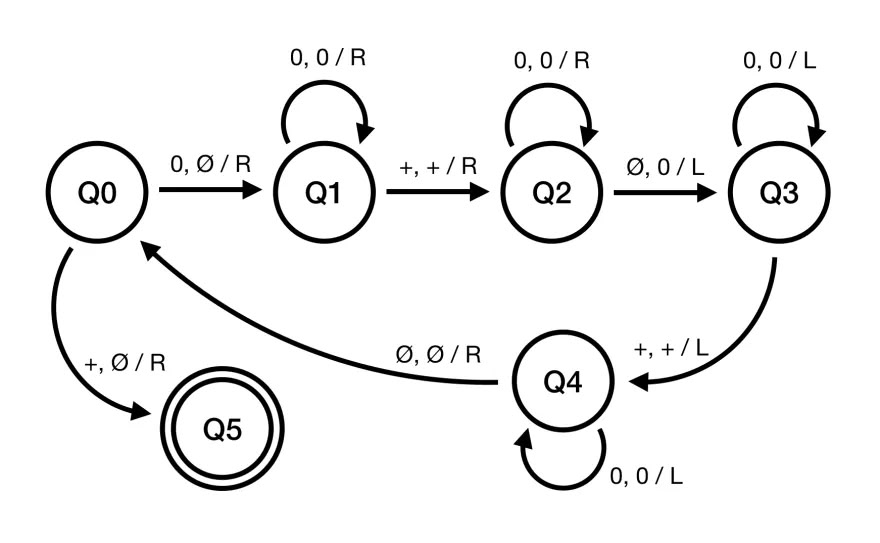
\includegraphics[width=0.6\textwidth]{images/turing.jpg}
    \centering
    \bicaption{图灵机模型示意图。给定一个字符串“00+000”(2 + 3),它将输出“000000”(5)。}{Turing machine model diagram. Given the string "00+000" (2 + 3), it outputs "000000" (5).}
  \end{center}
  \vspace{-3ex}
\end{figure}

图灵机的强大之处在于其普适性。尽管其结构看似简单,但它能模拟任何现代计算机程序(只要该程序能够在有限时间内完成计算)。这一特性被称为\textbf{图灵完备性}。换句话说,任何能够被算法解决的问题,都可以通过一台图灵机来模拟和计算。

图灵机不仅为我们理解什么是“可计算的”提供了精确的数学定义,也为计算机科学奠定了坚实的理论基础。它帮助我们区分了可判定问题(\textit{Turing-decidable problems},即存在图灵机能够总是停机并给出答案的问题)和不可判定问题(\textit{Turing-undecidable problems},即不存在这样的图灵机的问题,如停机问题)。在现代计算机设计中,虽然我们不再直接建造物理的图灵机,但其核心思想(即顺序执行指令、读写存储器、根据状态转换)依然深刻地影响着计算机体系结构和程序设计范式。理解图灵机,就是理解计算的本质极限和可能性。

\section{图灵机的理论局限性与NP问题}

尽管图灵机理论上具有强大的计算能力,但它也具有着一些根本性的局限。首先,在可判定性方面,图灵证明了著名的停机问题(\textit{Halting Problem})是不可解的。

\textbf{停机问题定义}:是否存在一个算法,可以判断任意程序 $\mathcal{P}$ 在输入 $\mathcal{I}$ 下是否会停止运行?

图灵使用对角线方法构造了一个自我引用的反例,证明没有任何图灵机能判断所有程序是否会停机\cite{turing1936computable}。因此,该问题被认为是不可判定问题(\textit{Undecidable Problem})的典型代表,同时也深刻说明了图灵机的能力并不涵盖“所有逻辑上可描述的问题”。

除了“是否可解”的问题之外,图灵机还面临“是否能有效求解”的限制。在“计算复杂性”层面,即便一个问题在理论上是可计算的,它也可能在实践中因为时间或空间资源限制而难以求解。这引出了对问题复杂度的分类。在学术界,计算复杂性理论将问题分为不同的类别,主要包括:

\begin{itemize}[noitemsep]
    \item \textbf{P类问题}:存在确定性多项式时间算法的问题。如果存在一个确定性图灵机算法可以在多项式时间内解决一个问题,该问题被称为P类问题。
    \item \textbf{NP类问题}:解可以在多项式时间内被验证的问题。NP (\textit{Non-deterministic Polynomial-time}) 是“非确定性多项式时间”的缩写。对于一个问题,如果给定一个候选解,我们可以在多项式时间内验证该解的正确性,那这个问题就被称为NP问题。即,对于一个NP问题,我们可以非确定性地猜测一个解,并在多项式时间内验证该解是否正确。
    \item \textbf{NP-Hard}:至少与NP中最难问题一样难的问题。NP难问题是指在非确定性多项式时间内无法解决的问题,它们不一定属于NP类,但可以被任何一个NP问题在多项式时间内约化。如果我们在多项式时间内能解决一个NP难问题,我们就可以在多项式时间内解决所有的NP问题。
    \item \textbf{NP-Complete}:既属于NP,又是NP-Hard的问题。如果我们能够在多项式时间内解决一个NP完全问题,那么我们可以在多项式时间内解决所有的NP问题,因为它们可以通过约化转换为NP完全问题。
\end{itemize}

形式化地,P 问题和 NP 问题可以被定义为:
\begin{equation}
\text{P} = \{\mathcal{L} \mid \exists \text{ 确定性图灵机 } \mathcal{M}, \text{ 使得 } \mathcal{M} \text{ 在 } \text{poly}(n) \text{ 时间内接受 } \mathcal{L}\}
\end{equation}

\begin{equation}
\text{NP} = \{\mathcal{L} \mid \exists \text{ 非确定性图灵机 } \mathcal{M}, \text{ 使得 } \mathcal{M} \text{ 在 } \text{poly}(n) \text{ 时间内接受 } \mathcal{L}\}
\end{equation}

最经典的问题是计算复杂性理论中的核心未解难题:

\begin{equation}
\text{P} \stackrel{?}{=} \text{NP}
\end{equation}

该问题是克雷数学研究所列出的七个“千禧年难题”之一\cite{ClayMath_PNP}。如果能够找到一个多项式时间算法来解决任何一个NP完全问题,那么意味着$P=NP$,即所有的NP问题可以在多项式时间内解决。然而,目前尚未找到证据来证明$P=NP$或$P\ne NP$,这仍然是计算机科学中一个重要的未解决问题。因此,即使一个问题是图灵可计算的,也可能由于指数级的时间复杂度而在实际中无法求解,即“理论上可计算 $\ne$ 实际上可行”。

\begin{figure}[h]
  \begin{center}
    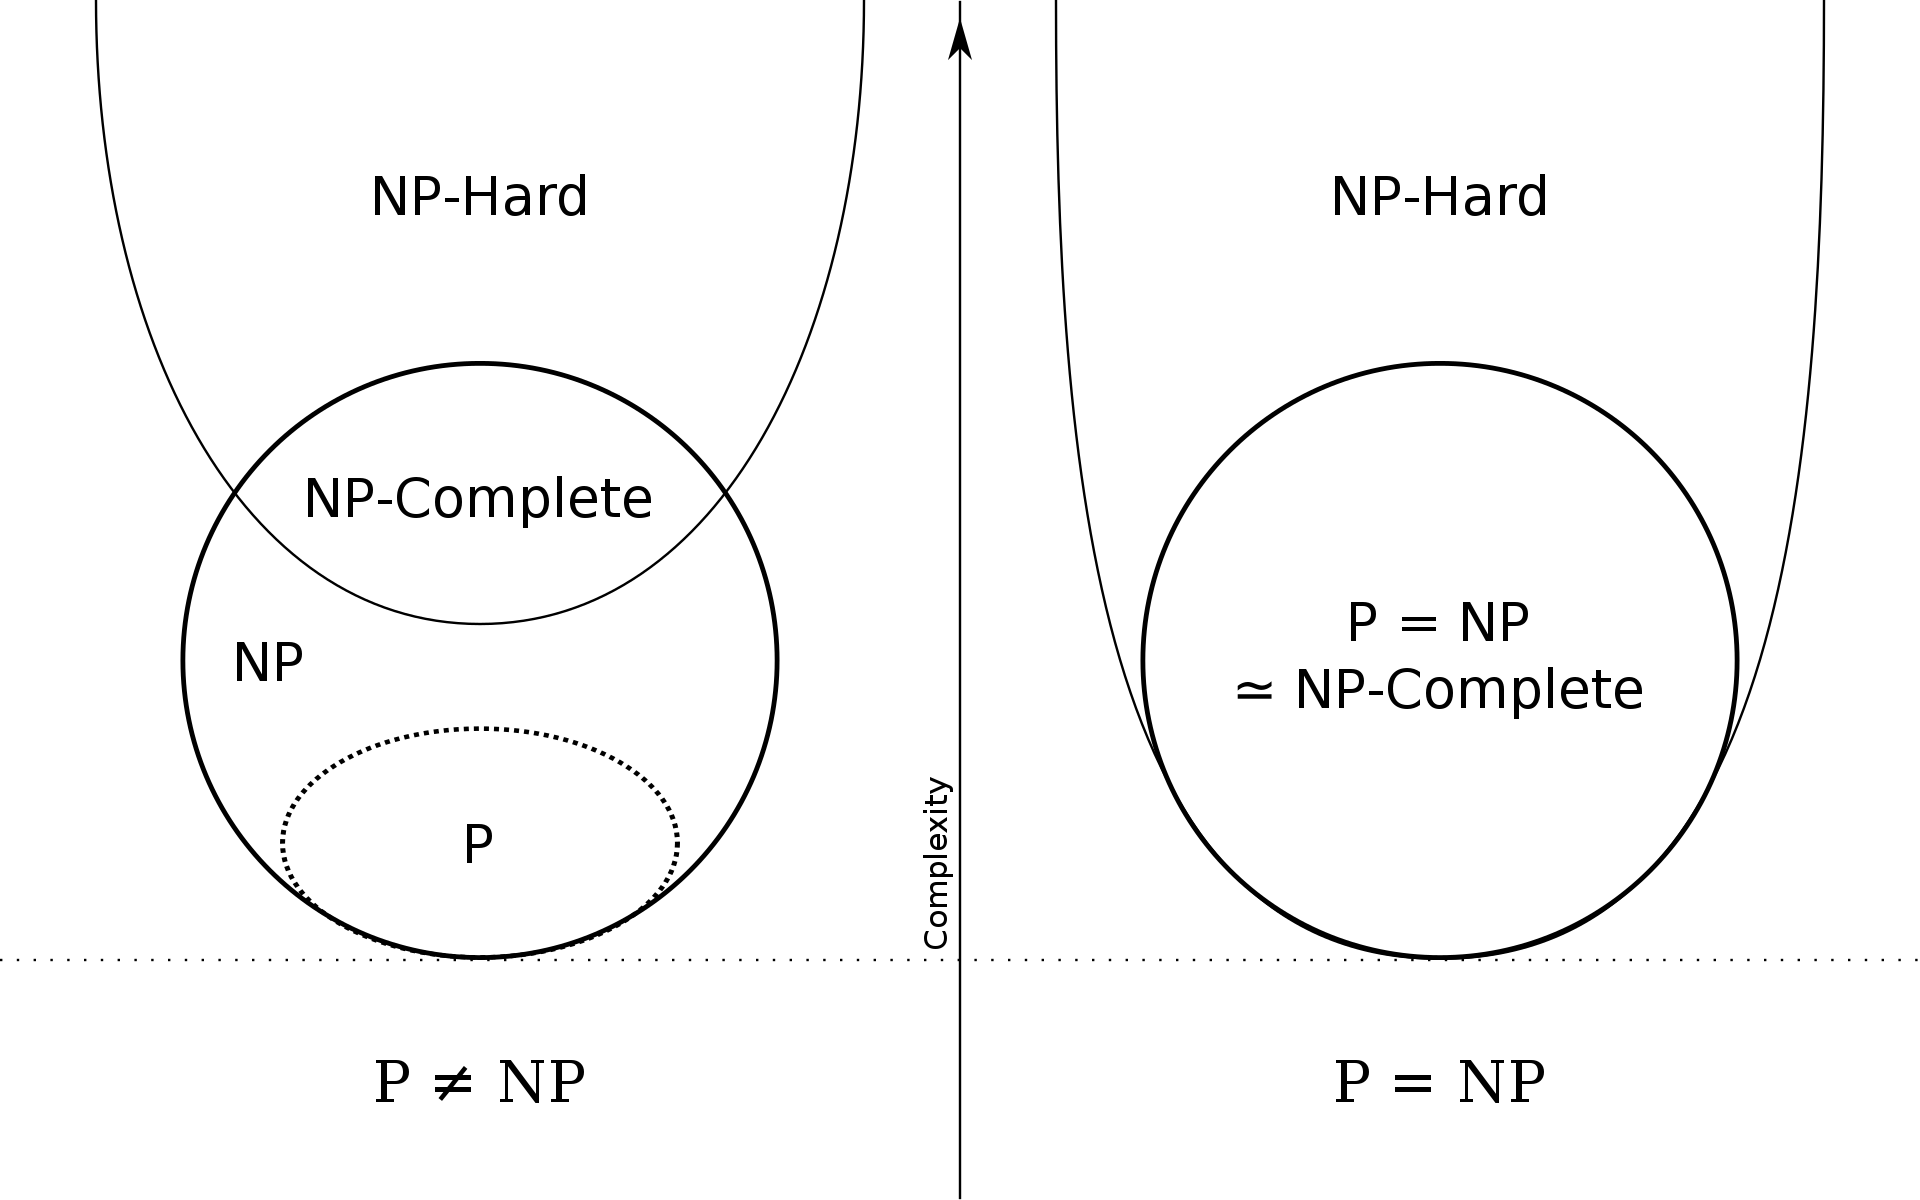
\includegraphics[width=0.5\textwidth]{images/pandnp.png}
    \centering
    \bicaption{P问题、NP问题、NP难问题与NP完全问题的欧拉图}{Euler diagram of P problems, NP problems, NP-hard problems, and NP-complete problems.}
  \end{center}
  \vspace{-3ex}
\end{figure}

\section{旅行商问题}

为了直观理解NP问题的求解困难程度,我们以经典的旅行商问题(\textit{Traveling Salesman Problem},TSP)为例加以说明。

\textbf{问题描述}:如图~\ref{fig:tsp}所示,旅行商问题要求在 $n$ 个城市中寻找一条总路径长度 $\mathcal{D}$ 最短的路线,使得每个城市仅访问一次,最终返回起点城市。在图论中,这一问题可以转化为:在一个加权的完全图$G = (V, E)$中(其中顶点代表城市,即$V = \{v_1, v_2, \ldots, v_n\}$,边表示城市之间的路径,即$E \subseteq V \times V$,边的权重$d: V \times V \rightarrow \mathbb{R}$对应路径的代价或距离),寻找一条哈密尔顿回路$C = (v_{\pi(1)}, v_{\pi(2)}, \ldots, v_{\pi(n)}, v_{\pi(1)})$,其中 $\pi$ 是 $1...n$ 的一个排列,来满足:

\begin{equation}
\mathcal{D} = \min_{\pi \in S_n} \sum_{i=1}^{n} d(v_{\pi(i)}, v_{\pi(i+1)}), \quad v_{\pi(n+1)} = v_{\pi(1)}
\end{equation}

\begin{figure}[h]
  \begin{center}
    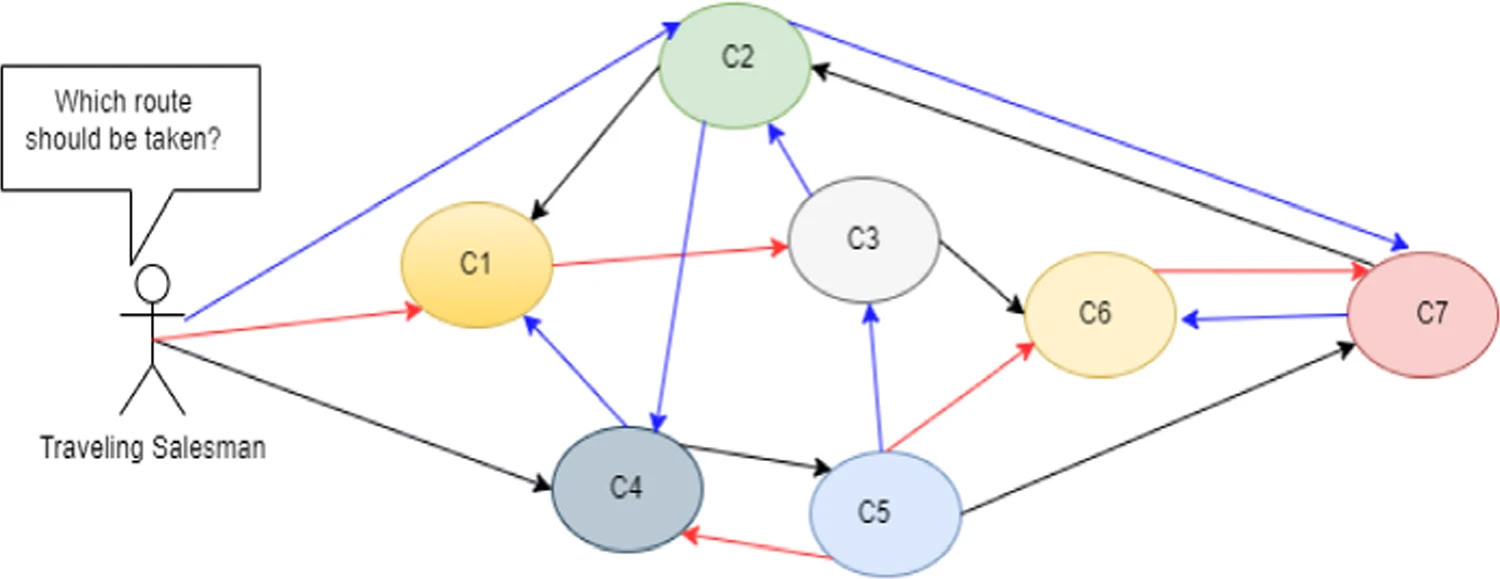
\includegraphics[width=0.7\textwidth]{images/tsp.jpg}
    \centering
    \bicaption{旅行商问题示意图,展示城市节点与路径路线图。}{Illustration of the Traveling Salesman Problem (TSP). It shows city nodes and path route maps.}
    \label{fig:tsp}
  \end{center}
  \vspace{-3ex}
\end{figure}

旅行商问题(TSP)是一个经典的组合优化问题,其目标是在一组城市中寻找一条最短的路径,使得每个城市仅访问一次,最后回到起点。为了解决这一问题,研究人员提出了多种算法,包括暴力枚举、贪婪策略、最近邻法、2-近似算法等,以及启发式和元启发式方法。我们查阅了相关文献,将这些方法的类型和时间复杂度整理在表~\ref{tab:tsp_methods}。

\begin{table}[H]
  \centering
  \bicaption{旅行商问题的求解方法}{Methods for solving the TSP.}
  \label{tab:tsp_methods}
  \begin{tabular}{ccc}
    \toprule
    \textbf{算法} & \textbf{类型} & \textbf{时间复杂度} \\
    \midrule
    Brute Force / Exhaustive Search\cite{cormen2022introduction} & 精确 & $O(n!)$ \\
    Dynamic Programming (Held-Karp)\cite{held1962dynamic} & 精确 & $O(n^2 2^n)$ \\
    Cutting Plane / Branch-and-Cut (Concorde)\cite{applegate2006traveling} & 精确 & $O(n! \cdot \text{poly}(n))$ or $O(2^{\text{poly}(n)})$ \\
    Nearest Neighbor Algorithm\cite{cormen2022introduction} & 启发式 & $O(n^2)$ \\
    Christofides Algorithm\cite{christofides2022worst} & 近似解 & $O(n^3)$ \\
    Lin-Kernighan-Helsgaun (LKH)\cite{lin1973effective} & 启发式 & $O(n^3)$ \\
    Ant Colony Optimization (ACO)\cite{dorigo1996ant} & 元启发式 & $O(k \cdot n^2)$ \\
    Genetic Algorithms (GA)\cite{holland1992adaptation} & 元启发式 & $O(k \cdot p \cdot n^2)$ \\
    Simulated Annealing\cite{kirkpatrick1983optimization} & 元启发式 & $O(k \cdot n^2)$ \\
    \bottomrule
  \end{tabular}
\end{table}

暴力枚举法通过遍历所有可能的城市访问顺序来寻找最优解,尽管结果精确,但其计算复杂度为 $O(n!)$,随着城市数量的增加,路径数量呈阶乘级增长,导致在实际应用中几乎不可行\cite{cormen2022introduction}。相比之下,贪婪算法和最近邻启发法\cite{cormen2022introduction}是基于局部最优选择构建路径的启发式策略,它们通常通过在每一步选择当前最近的未访问城市来扩展路径,虽然计算效率较高,但不能保证得到最优解。2-近似算法\cite{christofides2022worst}则通过构造最小生成树来构建近似的哈密尔顿回路,其路径长度上界为最优解的两倍。此外,还有一些启发式和元启发式方法,如遗传算法\cite{holland1992adaptation}、模拟退火\cite{kirkpatrick1983optimization}等,它们利用问题结构特性在解空间中进行智能搜索,以期在合理时间内获得接近最优的解。

然而,TSP被证明是一个NP完全问题,虽然可以在多项式时间内验证一个解是否可行,但当前尚无已知算法能在多项式时间内求得最优解。城市数量每增加一个,计算复杂度便呈指数级上升,导致求解时间迅速增长。即便使用最先进的算法与硬件资源,对于大规模实例,找到最优解依然十分困难,甚至在实际应用中常常无法实现。

这一“快速不可解”的本质不仅体现了图灵可计算问题在资源受限下的局限,也对计算机系统设计和算法研究提出了严峻挑战。在实际应用中,如路径规划、任务调度、资源分配等问题往往都涉及NP完全问题,因此必须在解的精度与计算时间之间做出权衡。

\chapter{人工智能的迅速发展是否突破了图灵机模型的局限?}
\label{sec:AI_breakthrough}

在近年来的技术浪潮中,人工智能以其在图像识别、自然语言处理、博弈策略等多个领域的突破,引发了人们对传统计算系统边界的重新思考。同时,在最近的几年里,以 ChatGPT 为代表的生成式人工智能系统,其表现出的语言理解与生成能力,使部分研究者开始质疑:AI是否已经超越了传统图灵机模型的理论边界?本章,我们从 AI 技术的演化出发,探讨其与图灵模型之间的内在关系。

\section{人工智能发展的演进}
\subsection{卷积神经网络}

卷积神经网络(\textit{Convolutional Neural Network}\cite{lecun2002gradient}, CNN)是深度学习领域的重要里程碑。CNN的核心思想在于通过模拟生物视觉皮层的局部感受野和权值共享机制,在捕获局部特征的同时大幅降低模型参数数量,从而有效应对高维度数据的处理挑战。其核心结构包括卷积层、池化层与全连接层。卷积层通过学习到的卷积核对输入数据进行特征提取;池化层则对提取到的特征进行降采样,以减少数据维度并增强模型的平移不变性;全连接层在网络末端对所有局部特征进行整合,用于最终的分类或回归任务。其中,卷积操作的数学表达式为:

\begin{equation}\vspace{-4ex}
y = f(\mathbf{W} * \mathbf{x} + b)
\end{equation}\vspace{-1ex}

其中 $\mathbf{W}$ 为卷积核,$*$ 表示卷积操作,$f$ 为激活函数(如ReLU),$\mathbf{x}$ 为输入特征图。CNN 在图像分类、目标检测等任务中表现出色,尤其擅长处理具有网格状拓扑结构的数据,如图像、视频和语音信号,成为计算机视觉领域的主流方法。

\subsection{AlphaGo 与强化学习}

AlphaGo\cite{silver2016mastering}是Google DeepMind开发的一个里程碑式的人工智能程序,它在围棋这一复杂博弈领域首次击败了人类世界冠军,这在很大程度上得益于其对深度强化学习(\textit{Deep Reinforcement Learning}, DRL)的创新性应用。 强化学习是一种通过智能体与环境的交互来学习最优决策策略的机器学习范式。智能体通过接收环境的奖励信号来调整自身行为,从而最大化长期累积奖励,达到强化学习的目的。AlphaGo的核心架构正是在卷积神经网络(CNN)强大的模式识别能力基础之上,结合了蒙特卡洛树搜索(MCTS)和强化学习方法。它使用基于CNN的深度策略网络来预测下一步棋的走法,以及同样基于CNN的深度价值网络来评估当前局面的胜率,从而有效剪枝搜索空间并指导MCTS的决策过程。强化学习框架形式化为:

\begin{equation}\vspace{-4ex}
\pi^* = \arg\max_\pi \mathbb{E} \left[ \sum_{t=0}^{\infty} \gamma^t R(s_t, a_t) \right]
\end{equation}\vspace{-1ex}

其中 $\pi$ 为策略函数,$R(s_t, a_t)$ 是状态 $s_t$ 下动作 $a_t$ 的即时奖励,$\gamma$ 是折扣因子,表示未来奖励的衰减。AlphaGo 的成功不仅展示了深度学习与强化学习的强大结合能力,也为复杂决策问题提供了新的解决思路。

\subsection{Transformer 与 ChatGPT}

Transformer\cite{vaswani2017attention} 是当前自然语言处理(Natural Language Processing, NLP)领域的主流架构,其设计初衷是为了克服循环神经网络(Recurrent Neural Network\cite{jordan1997serial}, RNN)在处理长序列时存在的长距离依赖问题和并行计算效率低下的缺点。 Transformer 摒弃了 RNN 的时序递归机制,完全依赖于自注意力机制(Self-Attention)来捕捉输入序列中不同位置之间的依赖关系。这种机制允许模型在处理序列的每个元素时,同时考虑到序列中的所有其他元素,从而更好地理解上下文信息。

\begin{equation}\vspace{-3ex}
\text{Attention}(Q, K, V) = \text{softmax}\left( \frac{QK^\top}{\sqrt{d_k}} \right) V
\end{equation}\vspace{-1ex}

其中, $Q$、$K$、$V$ 分别表示查询(Query)、键(Key)和值(Value)矩阵,$d_k$ 是键向量的维度。自注意力机制通过计算查询与键之间的相似度来加权值,从而生成新的表示。在此基础上,由OpenAI开发的ChatGPT(Chat Generative Pre-trained Transformer)实现了高水平的语言理解和生成能力。它通过在海量文本数据上进行预训练,学习了复杂的语言模式、语法结构以及世界知识,从而能够生成连贯、有逻辑且符合语境的文本。同时,ChatGPT结合了大规模预训练和指令微调等技术,使其能够执行翻译、问答、代码生成等多种复杂的自然语言任务,极大地推动了AI在NLP领域的进步。

\begin{figure}[h]
    \centering
    \begin{subfigure}[b]{0.40\textwidth}
        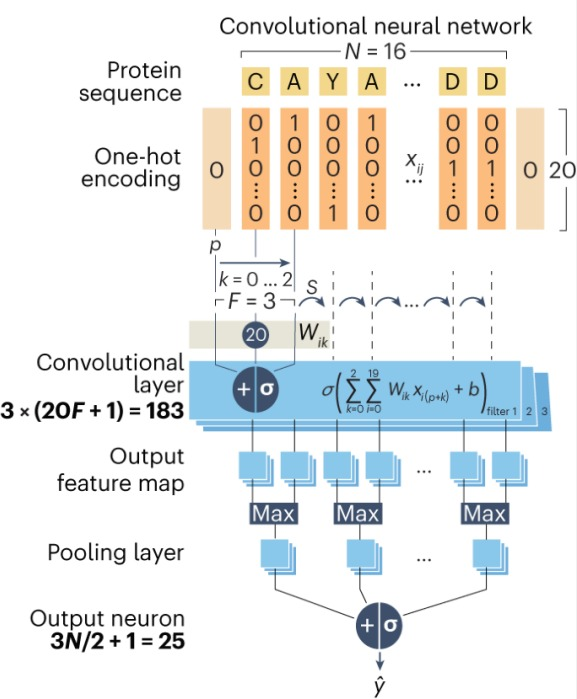
\includegraphics[width=\textwidth]{images/cnn.jpg}
        \caption{卷积神经网络示意图\cite{lecun2002gradient}}
        \label{fig:subimaga}
    \end{subfigure}
    \hfill
    \begin{subfigure}[b]{0.45\textwidth}
        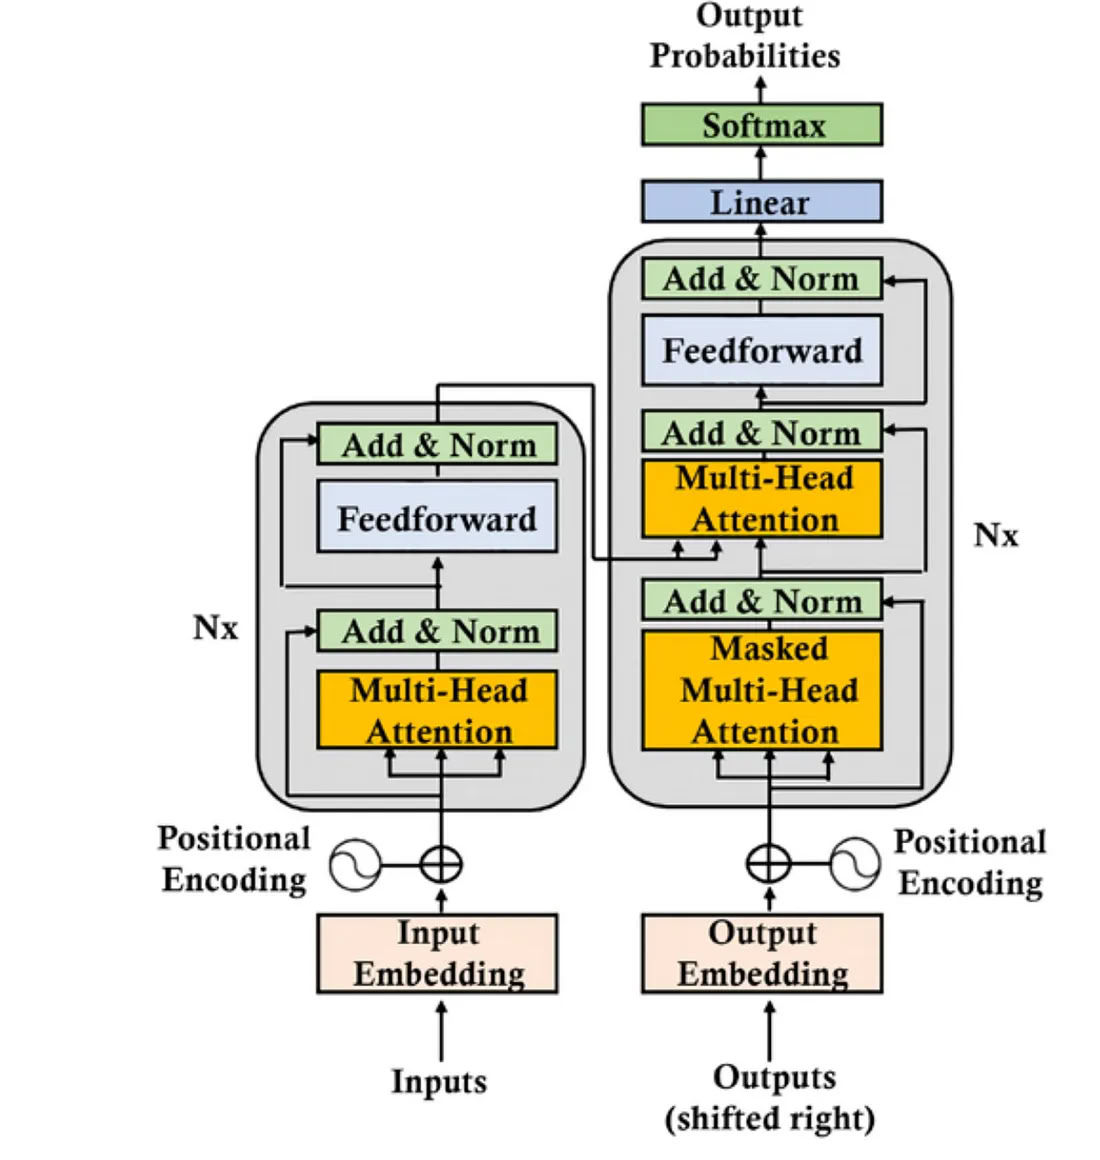
\includegraphics[width=\textwidth]{images/transformer.jpg}
        \caption{Transformer 模型示意图\cite{vaswani2017attention}}
        \label{fig:subimagb}
    \end{subfigure}
    \bicaption{卷积神经网络与 Transformer 模型示意图。}{Illustration of Convolutional Neural Network and Transformer model.}
    \label{fig:twoimages}
    \vspace{-3ex}
\end{figure}


\section{人工智能是否超越图灵模型?}

尽管现代人工智能(AI)系统展现出强大的拟人智能能力,其核心计算过程至今仍运行在传统图灵机等价架构之上。这具体体现在它们依赖于冯·诺依曼体系结构的计算机,并广泛利用图形处理器(GPU)或张量处理器(TPU)进行大规模并行浮点数运算。我们从计算理论的角度讨论,可以明确以下两点:

\begin{itemize}[noitemsep, topsep=0pt]
  \item 所有神经网络结构(包括复杂的Transformer架构)均可严格形式化为有限状态图与数值矩阵操作的组合。这些操作在计算上是离散的、可有限描述的,因此,\textbf{神经网络的计算过程完全属于图灵可计算的范畴。}
  \item 所有训练过程和推理过程,从数据输入、模型参数更新到最终结果输出,皆可在图灵完备的编程语言(如Python结合TensorFlow或PyTorch等深度学习框架)中实现和模拟。\textbf{这进一步证实了AI的计算本质未超出图灵可计算性理论的边界。}
\end{itemize}

尽管AI系统在规模上空前庞大,并在性能上取得了惊人的突破,但其本质依然牢固地限定在传统可计算性框架之内。更准确地说,当前AI的显著成功是这些因素协同作用的结果:

\begin{enumerate}[noitemsep, topsep=0pt]
 \item 首先,随着互联网等技术的普及,数据的规模呈指数级提升。训练数据集的规模从GB级跃升至PB甚至EB级别,为模型学习复杂模式提供了充足养料。
 \item 其次,硬件的性能呈飞跃式发展,以GPU和TPU为代表的并行计算硬件,其吞吐量和能效比大幅提升,使得大规模深度学习模型的训练成为可能。
 \item 第三,神经网络结构往往结合一些现代(\textit{State-of-the-art}, SOTA)的优化算法,优化算法迭代速度十分迅速,诸如Adam优化器、Layer Normalization、Dropout等高效且鲁棒的优化与正则化技术,显著提升了模型训练的稳定性和收敛速度。
 \item 最后,模型训练工程趋向于更加复杂的系统结构,包括大规模分布式训练框架、模型并行与数据并行策略、以及参数量化与模型剪枝等技术,极大地优化了AI系统的部署与运行效率。
\end{enumerate}

综上所述,\textbf{当前人工智能的能力提升,是在图灵计算范式下进行的一场“工程级扩展”和“规模化实现”,而非对图灵计算理论边界的突破。}AI的成就更多体现了在现有计算框架内,通过资源、算法和工程的优化所能达到的极限。

\chapter{AI的局限性:知识边界与黑箱模型}
\label{sec:AI_explainability}

尽管人工智能技术在过去十年取得了显著突破,其在语言理解、图像识别、博弈策略等任务中超越人类平均水平,但从更深层次的理论视角来看,当前人工智能仍然无法摆脱传统计算模型的基础约束,尤其是图灵机模型所揭示的根本局限性。本章将从 AI 的知识获取方式、可解释性问题、以及其行为不可预测性三个方面,系统讨论人工智能的内在限制,并进一步探讨这些限制是否构成一种新的计算边界。

\section{知识边界:AI 不能超越人类知识的“叠加”}

现阶段的主流人工智能系统(如 ChatGPT、AlphaFold 等)在技术实现上,本质上是一种高度复杂的统计归纳与模式匹配机制,其基础是对大规模人类知识语料的学习与压缩。即便采用自监督学习或强化学习技术,其本质仍是对既有信息的建模与泛化。

换句话说,AI 并不具备真正意义上的“创造性”,其所谓的“创新”行为,往往是不同语料片段、概念路径或语义关联的“组合”或“重组”。这种能力是广义的归纳,而非演绎意义上的新知识产生。

同时,AI 的运行仍然完全依赖图灵完备的可计算系统。无论是神经网络的训练算法,还是语言模型的推理过程,均可在经典图灵机架构中表达。换句话说,当前的 AI 仅在传统可计算问题的空间中“高效地游走”,并未跳出图灵计算模型的理论界限。以旅行商问题(TSP)为例,虽然 AI 可以基于启发式搜索提供近似解,但它依然无法从根本上规避该问题的 NP 难性质。尽管深度强化学习等方法可生成近似策略,但精确解的计算复杂度依旧为指数级。AI 只能在图灵模型允许的空间内优化,而无法“超越”。

人工智能的创新边界,仍受限于图灵机可计算的框架和人类知识的范式;AI 的强大并不意味着它具备突破不可计算性或NP难度的能力。

\section{黑箱模型:不可解释性与不可预测性}

现代人工智能系统,特别是大规模深度神经网络模型,普遍面临“黑箱性”(\textit{Black-box nature})的挑战。这种特性源于模型参数的巨量、学习机制的高度非线性以及复杂的输出行为,使得我们难以对其决策过程进行清晰的解释和全面的验证。传统软件工程中,系统的可验证性(Verifiability)和可预测性(Predictability)是核心质量标准;然而,AI系统的行为不再依赖显式规则和逻辑结构,而是基于“统计意义上的最优输出”,这为系统安全和可靠性评估带来了挑战。AI的不可解释性主要体现在以下几个方面:

\begin{itemize}[noitemsep, topsep=0pt]
  \item 神经网络内部的决策路径不可追踪的,内部隐藏层维度过高(如 GPT-4 的$\#$(层数) > 100,$\#$(参数量) > 10$^{11}$),导致推理路径难以复现;
  \item 没有形式化方法可以应用于SOTA大模型,现有形式化方法(如模型检测、逻辑证明)难以有效应用于非离散状态空间的连续神经网络系统;
  \item 神经网络的输出有不可控的风险,训练数据中隐含的偏见可能被放大,形成不符合事实的输出。
\end{itemize}

除了不可解释性,现代AI系统还展现出显著的不可预测性,这在工程实践中构成了一种新型的“计算局限”。虽然从形式计算理论的角度看,AI系统的所有行为仍可被映射为图灵可计算函数的组合,并未引入任何理论上的“不可计算”问题,但其在实际运行中的非确定性输出和高度复杂行为,导致人类对其未来状态的预测能力显著下降。具体表现为:

\begin{itemize}[noitemsep, topsep=0pt]
  \item 上下文敏感性:相同输入在不同上下文中可能产生截然不同的输出;
  \item 参数微调的敏感性:模型微调或训练细节的变化,可能导致系统行为完全偏移;
  \item 涌现行为:模型越大,其行为越“涌现”,越不具可控性。
\end{itemize}

这种“非决定性”不同于传统概率算法中的随机性,它更多地体现为一种结构性的不透明性。它使得用户或开发者难以完全掌控AI系统的行为空间,甚至难以确切地定义其所有可能的状态和输出。当前,对于AI的不可预测性是源于模型复杂性超越人类认知能力的暂时性“技术困难”,还是一种更深层的、无法回避的“计算现象学”,学术界尚无定论。然而可以肯定的是:AI系统已对传统“完全可控、可理解”的计算系统范式提出了严峻挑战。\textbf{这种挑战虽然不属于理论计算边界的扩展,但无疑已构成工程实践中的“新型局限”。}

\chapter{结论}
\label{sec:conclusion}

计算机系统的局限性存在于深层的理论层面受限于可计算性与复杂性理论所揭示的根本边界。本文从图灵机模型出发,回顾其定义及重要的理论,如停机问题的不可判定性与 $P \stackrel{?}{=} NP$ 的未解问题。传统计算模型所面临的一大核心问题,即使存在某些问题即使可解,也无法在可接受的时间和资源范围内有效求解。

随着深度学习与生成式模型的快速发展,社会各界对于 AI 是否已经突破图灵计算模型的局限产生了广泛兴趣。本文在回顾 AI 发展历程后指出,现有人工智能系统仍然依赖于图灵完备的冯·诺依曼架构;其行为可被视为图灵机上的“可计算”过程。在理论意义上,AI 并未超越图灵模型。

本文也指出,人工智能在实践中的表现呈现出一种“边界模糊化”的特征。其泛化能力、不可预测性与不可解释性使人类很难掌控其运行机制,这种“黑箱”特性挑战了传统计算系统对可靠性与可验证性的要求。

当前人工智能的发展并未实质突破图灵机的理论边界,但其在复杂性、可解释性与系统设计上的挑战,已经构成一种实践意义上的“新局限”。理解与应对这种局限,会成为下一阶段计算系统理论与人工智能伦理研究的最重要的课题之一。

% \newpage

\bibliographystyle{gbt7714-numerical}
\bibliography{references}

\end{document}